\chapter{Экспериментальные результаты}\label{ch:ch4}

\section{Апробация ПАЗЛ-3D для исследования алюминиевого сплава системы Al-Mg-Si}\label{sec:ch4/sect1}

В настоящее время установка ПАЗЛ-3D прошла широкую апробацию на различных материалах. Исследовались исходные состояния ферритно-мартенситных сталей ЭК-181, ЧС-139 [ref], дисперсно-упрочненных оксидами сталей ODS Eurofer, KP-(1-4), 10Cr ODS, 13.5Cr ODS, Austenitic ODS, ЭП-450 ДУО, ЭП-823 ДУО [ref], никелевые супер-сплавы [ref],  высокоэнтропийные сплавы [ref], и др. В настоящей главе представлены резульаты аппробации АЗТ установки ПАЗЛ-3D для сплавов алюминия, экономно-легированных сталей ЧТО-ТО ЕЩЁ.

Для тестирования установки были выбраны многокомпонентные сплавы с хорошей теплопроводностью, содержащие в своей структуре образования с характерным размером от единиц до сотен нанометров. Выбранный сплав Al-Mg-Si обладает повышенной прочностью, пластичностью, коррозийной стойкостью и жаростойкостью. Для выбранного сплава использовались следующие параметры исследования: температура образца 50~К, мощность лазерного излучения с гармоникой 515 нм составляла 10 мВт, скорость сбора данных в ходе эксперимента поддерживалась в пределах от 100 до 500 атомов/сек. Выбранные параметры являются наиболее часто используемыми для АЗТ исследований алюминиевых сплавов.

На Рисунке \cref{fig:AlMgSi_mass} представлена основная часть масс-спектра, полученного в результате проведения атомно-зондового исследования. Среднее разрешение по массе на полувысоте пиков составляет 500 отн. ед.

\begin{figure}[htb]
	\centerfloat{
		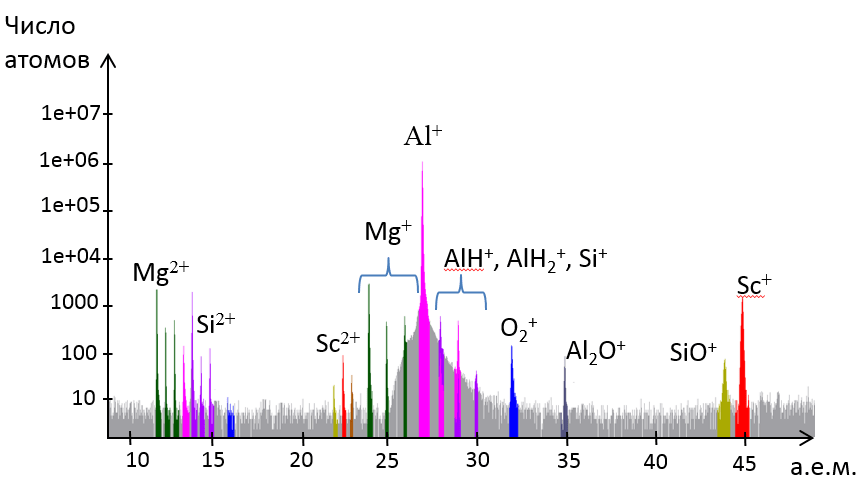
\includegraphics[width=.8\textwidth]{AlMgSi_mass}
	}
	\caption{Масс-спектр сплава Al-Mg-Sc (показана основная часть)\cite{scbibAlumYAFI}}
	\label{fig:AlMgSi_mass}
\end{figure} 
\FloatBarrier

На полученных атомных картах хорошо видны наноразмерные включения обогащенные Mg, Si, O и Cu. На Рисунке~\cref{fig:AlMgSi_3D}~(б) показаны атомные карты распределения Mg и Si. Включения Mg-Si имеют длину 50$\pm$10 нм и 10$\pm$2 диаметр. Поскольку включения имеют не сферическую форму, то для определения их концентраций использовались изо-концентрационные поверхности и проксиграммы. Химический состав матрицы и включений показан в Таблице \cref{tab:AlMgSi_table}. На Рисунке~\cref{fig:AlMgSi_3D}~(а) показаны изо-концентрационные поверхности Mg-Si 16~ат.~$\%$ (внутри таких поверхностей концентрация Mg-Si больше или равна 16~ат.~$\%$). Объемная плотность частиц составляет 2х$10^{22}$ см$^{-3}$.

\begin{figure}[htbp]
	\begin{minipage}[b][][b]{0.49\textwidth}\centering
		%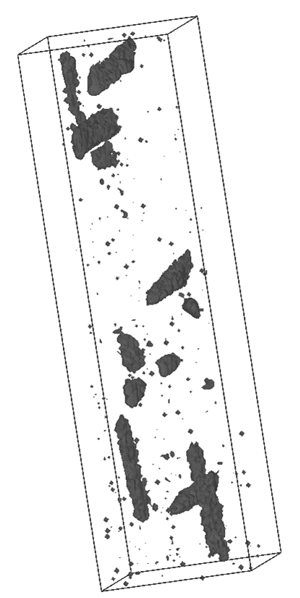
\includegraphics[width=\textwidth]{AlMgSi_3D_a} \\ а)
		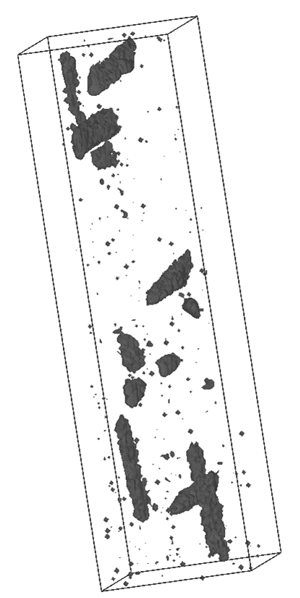
\includegraphics[scale=0.8]{AlMgSi_3D_a} \\ а)
	\end{minipage}
	%\hfill
	\begin{minipage}[b][][b]{0.49\textwidth}\centering
		%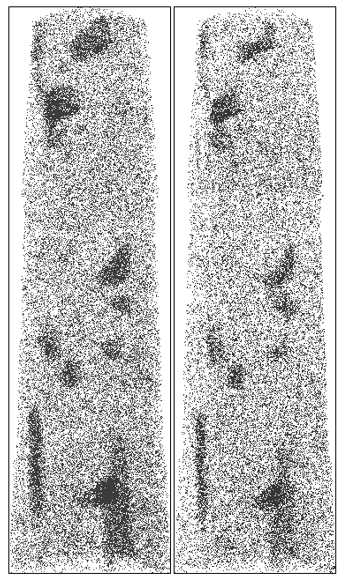
\includegraphics[width=\textwidth]{AlMgSi_3D_b} \\ б)
		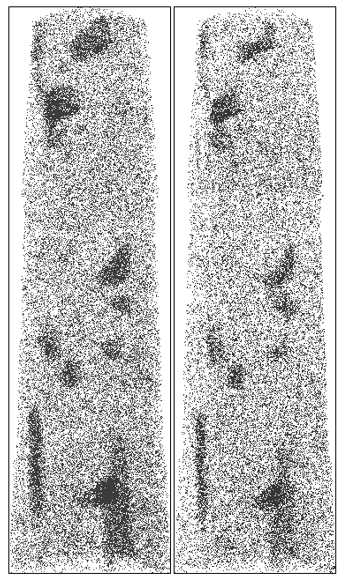
\includegraphics[scale=0.8]{AlMgSi_3D_b} \\ б)
	\end{minipage}
	\caption{а) Изоконцентрационные поверхности Mg и Si 16~ат.~$\%$, б) атомные карты распределения Mg (левый объем) и Si (правый объем). Размер исследованной области 47х47х167 нм$^3$}
	\label{fig:AlMgSi_3D}
\end{figure} 

\begin{table} [htbp]
	\centering
	%\begin{threeparttable}% выравнивание подписи по границам таблицы
	\caption{Состав матрицы и включений сплава Al-Mg-Si at. $\%$}%
	\label{tab:AlMgSi_table}%
	\begin{SingleSpace}
		\begin{tabular}{| c | c | c |}
			\hline
			Элемент & Матрица & Включения \\ \hline
			Al & 98.67 $\pm$ 0.01 & 67 $\pm$ 3 \\ \hline
			Mg & 0.56 $\pm$ 0.01 & 18 $\pm$ 3 \\ \hline
			Si & 0.35 $\pm$ 0.01 & 13 $\pm$ 2 \\ \hline						
			Cu & 0.03 $\pm$ 0.01 & 0.35 $\pm$ 0.03\\ \hline
			Остальные (O, S) & Баланс & Баланс \\ \hline			
		\end{tabular}%
	\end{SingleSpace}
	%\end{threeparttable}
\end{table}

Применение АЗТ для алюминиевого сплава типа Al-Mg-Si продемонстрирована возможность исследования с получение детальной информации о размерах и составе включений с характерным размером в десятки нанометров. Получены атомные карты распределений элементов в исследуемых объемах. Проведена оценка размеров и состава включений и матрицы материала.

\FloatBarrier

\section{Демонстрация возможности АЗТ по исследованию структуры среднеуглеродистой стали}\label{sec:ch4/sect2}

Для демонстрации возможностей АЗТ по исследованию промышленных высокопрочных износостойких сталей была выбрана среднеуглеррдистая сталь Б1700 (C 0.45, Si 0.36, Mn 1.13, Ni 0.67, Cu 0.63, Cr 1.26, Mo 0.40, Ti 0.03, V 0.06, Nb 0.02, Ca 0.03, B 0.003, S 0.008, P 0.005 масс.\%) в виде листового проката после отпуска при различных температурах. Основной целью было показать распределение углерода и легирующих элементов в объеме. В ходе исследований параметры работы установки поддерживались на следующих значениях: температура образца 40~К, мощность лазерного излучения гармоники 515~нм 1.5~мВт, скорость сбора данных от 60 до 500 атомов/сек.

Полученные атомные карты образца стали после отжига при 150 \textdegree С показаны на Рисунке \cref{fig:SteelAtomMaps1}, общий объем полученных данных составляет 23x23x200 нм$^{3}$. В Таблице \cref{tab:SteelComposition150} показан состав общий образца, состав матрицы и состав выделенных областей 1 и 2 на атомных картах.

\begin{figure}[ht]
	\centerfloat{
		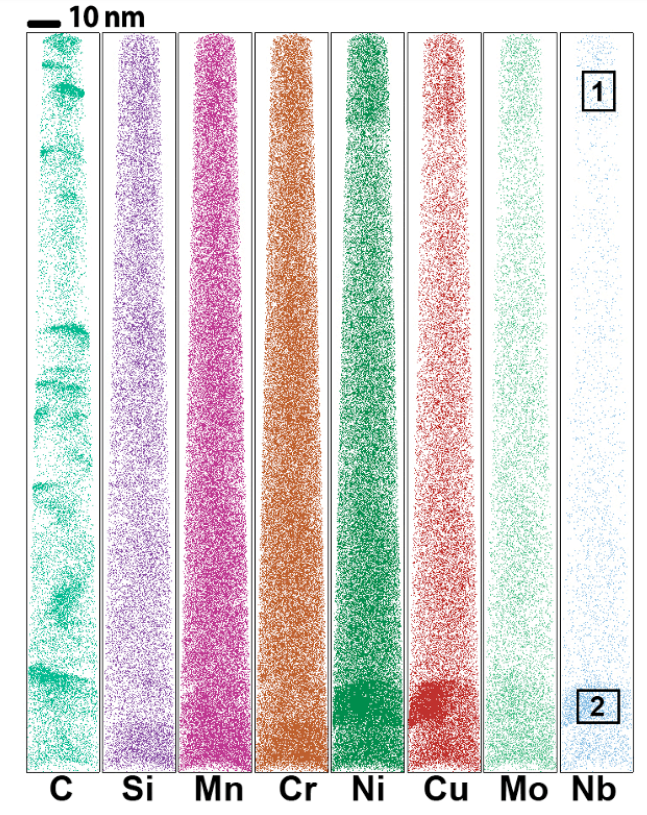
\includegraphics[width=.7\textwidth]{SteelAtomMaps1}
	}
	\caption{Атомные карты образца среднеуглеродистой стали после отпуска при 150 \textdegree С \cite{scbibRyabov}. Состав областей 1 и 2 показан в Таблице \cref{tab:SteelComposition150} }
	\label{fig:SteelAtomMaps1}
\end{figure} 

\begin{table} [htbp]
	\centering
	\caption{Состав стали, исследованного образца, матрицы и областей 1 и 2 среднеуглеродистой стали после отпуска при температуре 150 \textdegree С (at.\%)}%
	\label{tab:SteelComposition150}%
	\begin{SingleSpace}
		\begin{tabular}{|p{3cm}| c | c | c | c | c | c | c | c | c | c | c |}
			\hline
			& C & Si & Mn & Ni & Cu & Cr & Mo & Ti & V & Nb & Al     \\ \hline
			Состав массивного образца     & 0.45 & 0.36 & 1.13 & 0.67 & 0.63 & 1.26 & 0.40 & 0.03 & 0.06 & 0.02 & 0.04   \\ \hline
			Среднее по объему   & 0.45 & 0.42 & 1.11 & 0.49 & 0.62 & 1.37 & 0.23 & - & 0.07 & 0.10 & 0.04   \\  \hline		
			Матрица   & 0.26 & 0.41 & 1.09 & 0.38 & 0.46 & 1.34 & 0.19 & - & 0.07 & 0.05 & 0.05   \\  \hline	
			Область 1   & 0.97 & 0.53 & 1.31 & 0.49 & 0.51 & 1.54 & 0.32 & - & 0.08 & 0.12 & 0.09   \\  \hline
			Область 2   & 0.71 & 0.28 & 1.12 & 0.94 & 1.05 & 1.34 & 0.38 & - & 0.07 & 0.32 & 0.04   \\  \hline	
		\end{tabular}%
	\end{SingleSpace}
\end{table}

Для анализа локального распределения элементов построен профиль линейных концентраций вдоль всего образца (Рисунок \cref{fig:SteelLinear1}). По линейным концентрациям и атомным картам можно явно определить наличие областей с повышенным содержанием углерода, оценить их морфологию и состав. Средняя концентрация углерода в углеродных включениях составляет 1.5~ат.\%. Присутствует также сегрегация углерода, дополнительно обогащенная также никелем, ниобием и молибденом.

\begin{figure}[ht]
	\centerfloat{
		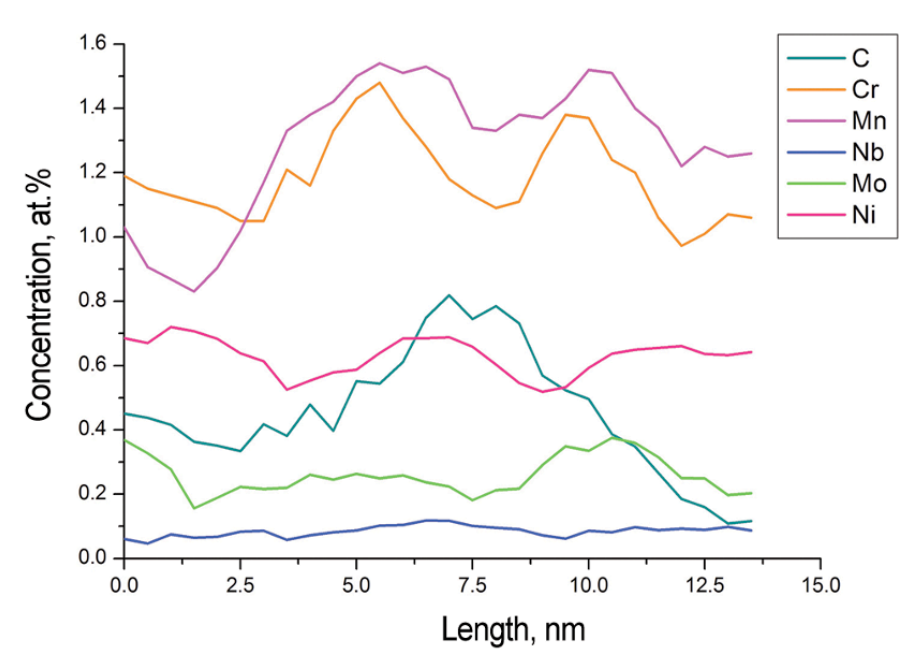
\includegraphics[width=.8\textwidth]{SteelLinear1}
	}
	\caption{Линейные профили концентраций для образца среднеуглеродистой стали после отпуска при 150 \textdegree С \cite{scbibRyabov}}
	\label{fig:SteelLinear1}
\end{figure}

\begin{figure}[htb]
	\centerfloat{
		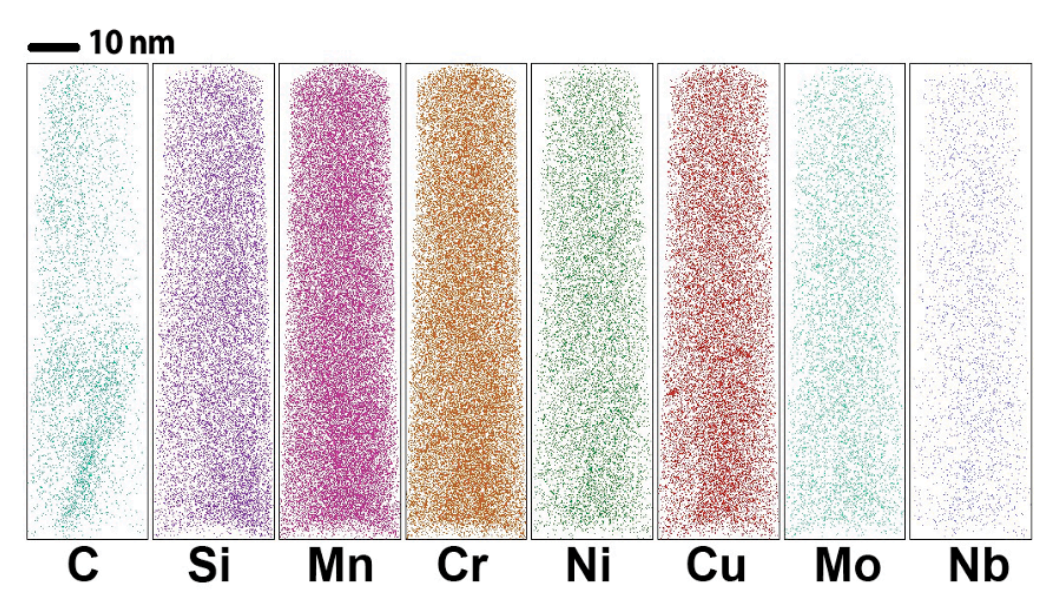
\includegraphics[width=.8\textwidth]{SteelAtomMaps2}
	}
	\caption{Атомные карты образца среднеуглеродистой стали после отпуска при 350 \textdegree С \cite{scbibRyabov}}
	\label{fig:SteelAtomMaps2}
\end{figure}

Для второго состояния материала (после отпуска при 350 \textdegree С) также получены атомные карты (Рисунок \cref{fig:SteelAtomMaps2}). Размер полученных данных составляет 25х25х100 нм$^{3}$. В Таблице \cref{tab:SteelComposition350} показан состав массивного образца и матрицы. Состав матрицы, без учета включений примерно соответствует составу массивного образца за исключением углерода, молибдена и ниобия. 

Для более детальной характериазции углеродного включения был построен отдельный линейный профиль концентрации для малого 3D объема (Рисунок \cref{fig:SteelLinear2}). На Рисунке \cref{fig:SteelAtomMapsLin} показана область, которая была выбрана для построения линейного профиля. Данный профиль наглядно демонстрирует обогащение углеродом границы зерна до 0.8~ат.\%, а также заметно обогащение по хрому и марганцу до 1.5~ат.\% каждый.

\begin{figure}[htb]
	\centerfloat{
		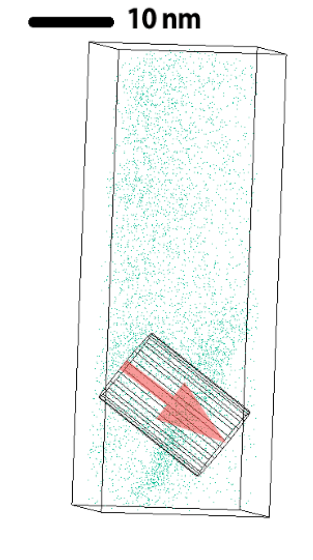
\includegraphics[width=.3\textwidth]{SteelAtomMapsLin}
	}
	\caption{Атомная карта распределения углерода образца среднеуглеродистой стали после отпуска при 350 \textdegree С \cite{scbibRyabov}. Показана область и направление построения линейной концентрации для границы зерна.}
	\label{fig:SteelAtomMapsLin}
\end{figure}

\begin{figure}[htb]
	\centerfloat{
		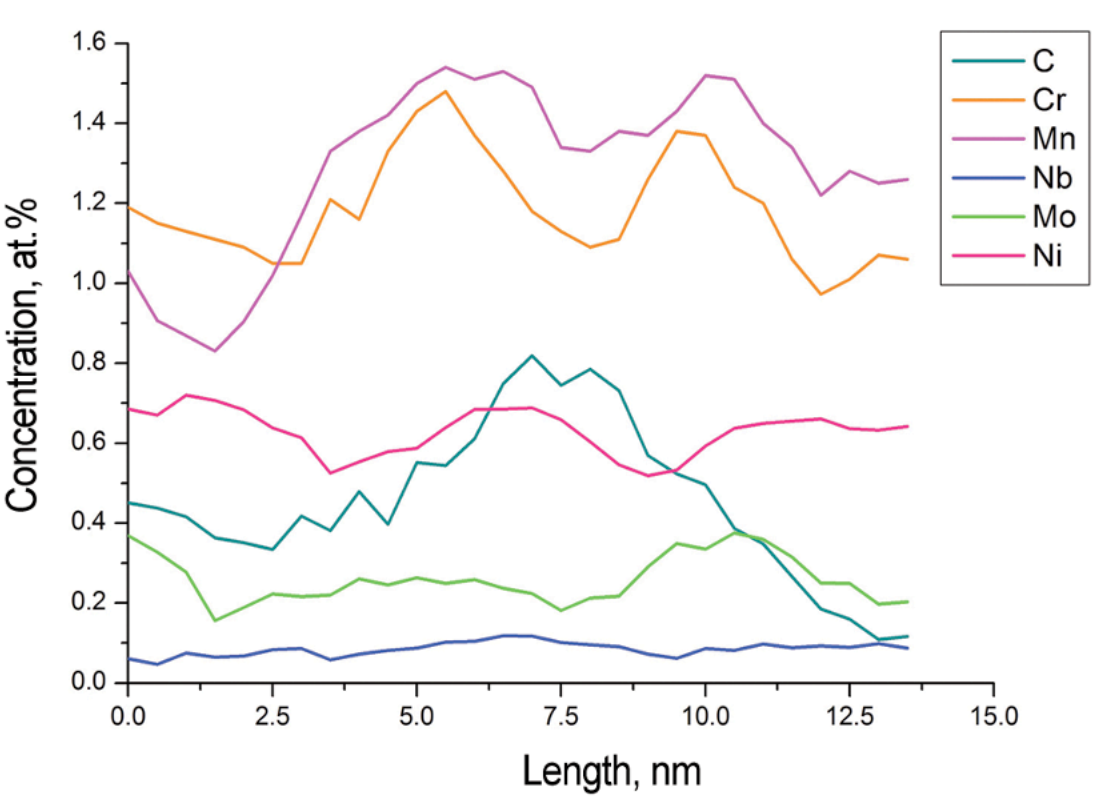
\includegraphics[width=.8\textwidth]{SteelLinear2}
	}
	\caption{Линейные профили концентраций для границы зерна образца среднеуглеродистой стали после отпуска при 350 \textdegree С \cite{scbibRyabov}}
	\label{fig:SteelLinear2}
\end{figure}

\begin{table} [htbp]
	\centering
	\caption{Состав стали, исследованного образца, матрицы и областей 1 и 2 среднеуглеродистой стали после отпуска при температуре 350 \textdegree С (at.\%)}%
	\label{tab:SteelComposition350}%
	\begin{SingleSpace}
		\begin{tabular}{|p{3cm}| c | c | c | c | c | c | c | c | c | c | c |}
			\hline
			& C & Si & Mn & Ni & Cu & Cr & Mo & Ti & V & Nb & Al     \\ \hline
			Состав массивного образца     & 0.45 & 0.36 & 1.13 & 0.67 & 0.63 & 1.26 & 0.40 & 0.03 & 0.06 & 0.02 & 0.04   \\ \hline
			Среднее по объему   & 0.37 & 0.41 & 1.16 & 0.61 & 0.57 & 1.37 & 0.23 & - & 0.07 & 0.10 & 0.05   \\  \hline		
			Матрица   & 0.37 & 0.40 & 1.14 & 0.60 & 0.55 & 1.35 & 0.22 & - & 0.07 & 0.10 & 0.05   \\  \hline		
		\end{tabular}%
	\end{SingleSpace}
\end{table}
\FloatBarrier
Исследования методом атомно-зондовой микроскопии позволили выявить многочисленные сегрегации атомов углерода в образце после отпуска при 150 \textdegree C. Полученные данные хорошо согласуются с данными просвечивающей электронной микроскопии: после отпуска при 150~\textdegree C наблюдались наиболее мелкие карбиды со средним размером 13~нм и объемной плотностью $2.2*10^{22} m^{-3}$ \cite{scbibRyabov}. Для состояния  с большей температурой отпуска 300 \textdegree C наблюдаются крупные частицы размером до 164–180~нм на границах реечного мартенсита и на границах исходных аустенитных зерен, где остаточный аустенит с объемной долей встречается и до 5\% \cite{scbibRyabov}.

\FloatBarrier

\section{Исследование изменения структуры высокопрочной экономнолегированной стали}\label{sec:ch4/sect3}

В качестве другого примера для апробации созданной установки ПАЗЛ-3D также были выбраны низкоуглеродистые стали. Одной из актуальных задач в разработке низкоугеродистых сталей является повышение уровня прочности и требуемой прокаливаемости при закалке \cite{scbibGlubev}. Данный класс материалов важен в разработке новых атомных ледоколов и морских технических средств добычи углеводородов. Для улучшения основных характеристик материала используются различные системы легирования. В процессе закалки или высокотемпературного отпуска может изменяться как микро, так и наноструктура материала. Соответственно, атомно-зондовая томография может предоставлять важную информацию о локальном распределении химических элементов в данных материала на различных этапах обработки.

Для демонстрации возможности АЗТ исследований использовалась сталь 09ХГН2МД. Состав стали мас. \%: 0.090 С; 0.30 Si; 0.70 Mn; 3.0 (Cr+Ni+Cu+Mo); 0.027 (V+Nb); 0.04 Al; 0.004 Ti; 0.002 Sn; 0.006 N; 0.003 S; 0.007 P. Были изучены три состояния,  состав образца и кластеров (при их наличии) показан в Таблице~\cref{tab:SteelComposition09X}. Исследование проводилось при следующих условиях: температура образца 40~К, мощность лазерного излучения при гармонике 515~нм 1.6~мВт, скорость сбора данных от 60 до 250 атомов/сек.

%\begin{itemize}
%	\item Закалка от 950 \textdegree C
%	\item Закалка от 950 \textdegree C + отпуск при 570 \textdegree С
%	\item Закалка от 950 \textdegree C + отпуск при 630 \textdegree С
%\end{itemize}

\begin{table} [htbp]
	\centering
	\caption{Состав образцов и кластеров для 09ХГН2МД (средние значения), ат.\%}
	\label{tab:SteelComposition09X}%
	\begin{SingleSpace}
		\begin{tabular}{| p{4.5cm} | c | c | c | c | c | c | c | c |}
			\hline
			 & & C & Si & Mn & Ni & Cr & Mo & Nb     \\ \hline
			\multirow{2}{*}{Закалка от 950 \textdegree C} & Образец & 0.19 & 0.53 & 0.71 & 0.85 & 0.59 & 0.13 & 0.01    \\ \cline{2-9}
			& Кластеры & 3.38 & 0.60 & 0.79 & 0.77 & 0.44 & 0.17 & 0.02    \\  \hline		
			Закалка от 950 \textdegree C + отпуск при 570 \textdegree С & Образец & 0.06 & 0.57 & 0.72 & 0.97 & 0.52 & 0.13 & 0.006    \\ \hline
			\multirow{2}{45mm}{Закалка от 950 \textdegree C + отпуск при 630 \textdegree С} & Образец & 0.09 & 0.54 & 0.70 & 1.08 & 0.50 & 0.18 & 0.007    \\ \cline{2-9}
			& Кластеры & 3.88 & 0.59 & 1.00 & 1.25 & 0.74 & 0.71 & -    \\  \hline	
		\end{tabular}%
	\end{SingleSpace}
\end{table}

\FloatBarrier
С помощью АЗТ показано, что в закаленном состоянии наблюдаются кластеры (наночастицы с повышенным содержание углерода), в которых содержание основных легирующих элементов практически не отличается от матрицы. Но после отпуска при температуре 570 \textdegree С в течении 3 часов происходит диссоциация кластеров. После отпуска при температуре 630 \textdegree С с помощью АЗТ были обнаружены кластеры с повышенным содержанием C, Mn, Cr и Mo (см. Таблицу \cref{tab:SteelComposition09X}). Наблюдаемые с помощью АЗТ эффекты подтверждены с помощью ПЭМ исследований \cite{scbibGlubev}.

В данном исследовании методика АЗТ помогла установить особенности изменения структуры стали 09ХГН2МД при высокотемпературном отпуске. Полученные данные могут быть применены в задаче оптимизации режимов термической обработки листового проката.

\FloatBarrier

\section{Исследование алюминия МИСиС Торгом}\label{sec:ch4/sect4}

Ожидает согласования с МИСиС Торгом

\FloatBarrier
\clearpage
\section{Основные результаты по главе 4}\label{sec:ch4/sect5}


В главе показаны возможности АЗТ установки ПАЗЛ-3D по исследованию материалов с нано-размерными особенностями. Продемонстрированы примеры визуализации АЗТ данных с помощью таких инструментов как: масс-спектры, атомные карты, линейные профили концентраций, изо-концентрационные поверхности и поиск кластеров. Продемонстрированный набор инструментов позволяет достаточно полно и подробно описывать кластеры/фазы в исследуемых материалах.

На примере исследования алюминиевого сплава типа Al-Mg-Si показана возможность изучения состава и структуры зон Гинье-Престона. Размер исследуемых зон может быть от нескольких нанометров до нескольких десятков нанометров. Также показана возможность программного обеспечения по визуализации нано-размерных объектов с помощью изо-концентрационных поверхностей.

Также в главе показаны исследования среднеуглеродистой стали Б1700. С помощью атомных карт показано распределение углерода в объеме образцов. Построены линейные профили концентраций химических элементов. Рассчитана объемная плотность карбидов в материале.


В рамках исследования высокопрочной экономнолегированной стали 09ХГН2МД показана возможность проводить поиск кластеров с определением их состава.




\FloatBarrier
\clearpage











%\nopagebreak - не разрывать страницами?







